%%%%%
% CH4 %
%%%%%

\chapter{Transient heat conduction}
	Let's Imagine that we want to cool a bottle of beer. What time will it take ? We will consider 3 different cases neglecting sometimes convection sometimes conduction. 
	
\section{Lumped systems analysis}
	\begin{wrapfigure}[6]{l}{3cm}
	\vspace{-5mm}
	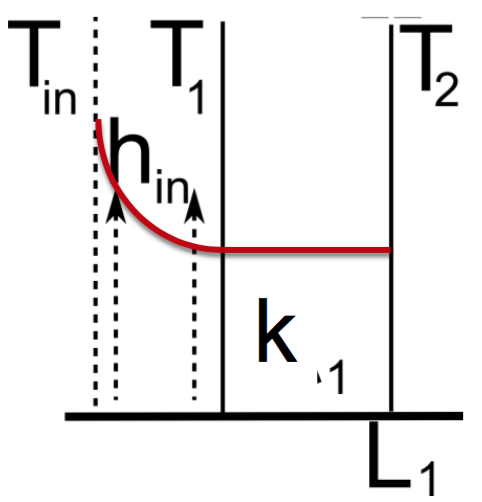
\includegraphics[scale=0.3]{ch3/8}
	\end{wrapfigure}	
	Let's study the case where convection is the limitative factor for heat (dispersion of heat within the solid is negligible compared to heat arrival to the surface). Let's remind the expression of the Biot number (go to \autoref{sec:3.3.3}). In this case, the $Bi \gg 1$
	\begin{equation}
		Bi = \frac{L_1h_{in}}{k_1}
	\end{equation}
	
	\subsection{Calculation of lumped systems}
		Let's consider an object of volume $V$ and surface $A$ initially to temperature $T_i$ that we put into an infinite temperature $T_\infty$ enviroment. We want to know what happens. So my accumulation, is equal to the amount that comes with the convection
		\begin{equation}
			V\rho c_p \frac{\partial T}{\partial t} = A h(T_\infty - T)
		\end{equation}
		Integrating and applying the initial condition $t = 0 \rightarrow T = T_i$
		\begin{equation}
			\underbrace{\frac{T-T_\infty}{T_i - T_\infty}}_{\theta} =
			 \exp \left( - \frac{Ah}{V\rho c_p}t \right) = 
			 \exp \left( - \underbrace{\frac{Vh}{Ak}}_{Bi} \underbrace{\frac{A^2k}{V^2\rho c_p}t}_{Fo} \right) 
		\end{equation}
It can always be expressed like a function of theta. 
The expression in the $\exp$ must be undimentional so we will make it appear. $V/A$ = lenght, so the definition of Biot number appears. The other is including t and is called the \textbf{Fourrier number}. 

	\subsection{Fourrier number}
		\begin{equation}
			\theta = \exp (-Bi \, Fo) \qquad Fo = \frac{A^2k}{V^2 \rho c_p}t = \frac{A^2\alpha }{V^2}t
		\end{equation}
		If we look to the units, we see that it's the undimentionnal time of the process. It compares the time since the external temperature change and the characteristic time of heat conduction in the object. 
		
\section{Semi-infinite solid}
	\subsection{Error function}
		\begin{wrapfigure}[7]{l}{2.8cm}
		\vspace{-5mm}
		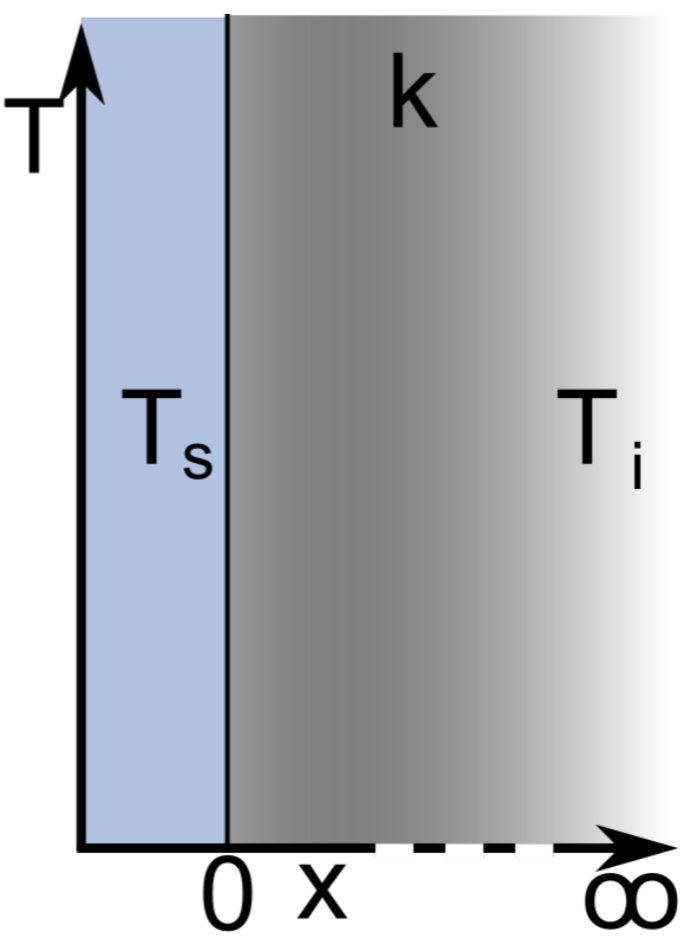
\includegraphics[scale=0.2]{ch4/2}
		\end{wrapfigure}	
		This is the case within the conduction only appear on a small franction of the total solid and an infinite surface is in contact with a fluid. The $Bi \ll 1$. We respect equation without source term 
		\begin{equation}
			\frac{\partial T}{\partial t} + \alpha \frac{\partial ^2 T}{\partial x^2 }
		\end{equation}
		We don't do the calculus in the course but after integrating and applying the conditions $T = T_S$ for $x=0$ $\forall t \leq 0$, $T = T_i$ for $x\rightarrow + \infty$ and $T = T_i$ for $t=0$ $\forall x > 0$, we obtain the result 
		\begin{equation}
			\frac{T-T_S}{T_i-T_S} = erf(\eta ) \qquad with \qquad \eta = \frac{x}{\sqrt{4\alpha t}} \qquad and \qquad erf(\eta ) = \frac{2}{\pi} \int _0 ^\eta \exp (-u^2) \, du
		\end{equation}
		
		\begin{wrapfigure}[7]{r}{2.8cm}
		\vspace{-5mm}
		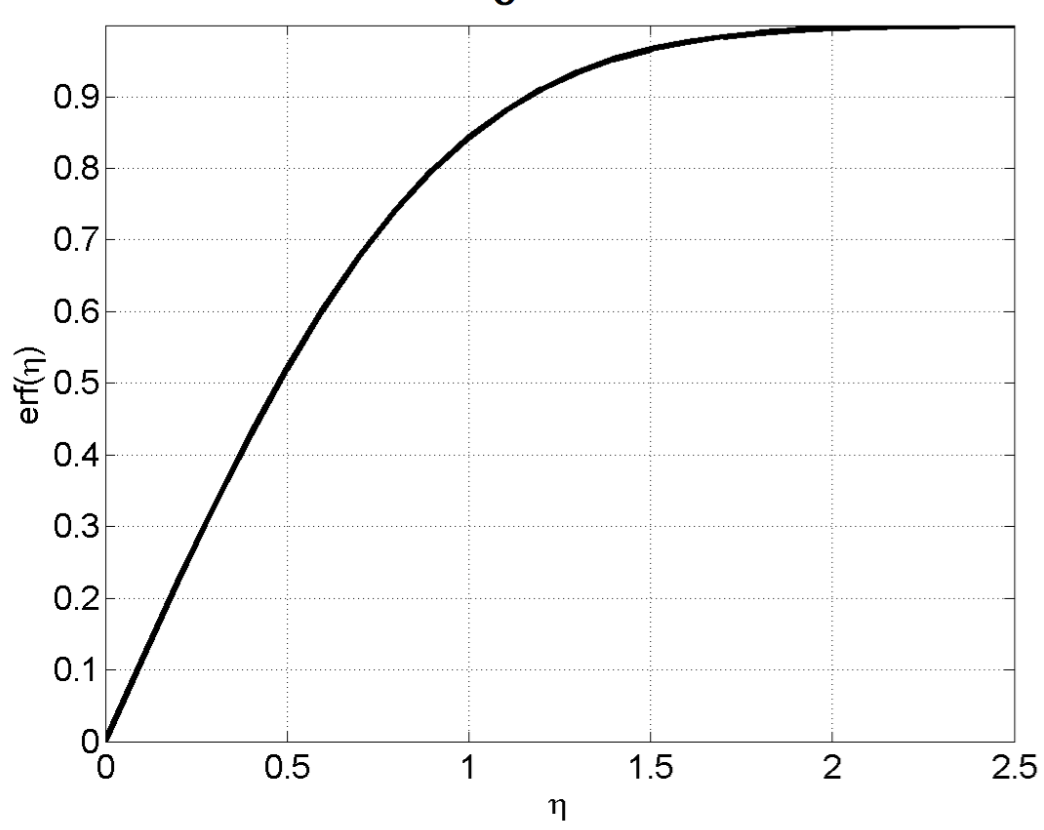
\includegraphics[scale=0.2]{ch4/3}
		\end{wrapfigure}	
		We see that $\eta$ combines position and times. You progress in the object proportionallly to the square root of time. A fixed value of $\eta$ means a fixed value of temperature. The flux density is expressed 
		\begin{equation}
			\dot{q} = -k \frac{\partial T }{\partial x }| _{x=0} = k \frac{T_S-T_i}{\sqrt{\pi \alpha t}}
		\end{equation}
Im assuming an infinite body, is it realistic ? where does my heat go ?

	\subsection{Penetration lenght}
		
	
	